\documentclass[12pt,a4paper]{article}
\usepackage{algorithm, algpseudocode, amsmath, amssymb, amsthm, bm, csquotes, emf, empheq, geometry, graphicx, hyperref, listings, mhchem, multirow, siunitx, slashbox, subcaption, upgreek}
\usepackage[italicdiff]{physics}
%\usepackage[section]{placeins}
\usepackage[justification=centering]{caption}
\usepackage[column=O]{cellspace}
\usepackage[extrafootnotefeatures]{xepersian}
\hypersetup{colorlinks=true, urlcolor=cyan}

\title{کدری جو}
\author{آرتین خانعلی، سپهر سلمانی یگانه، صالح شاملو احمدی\\\\
	آزمایشگاه نجوم، ترم تابستان ۱۴۰۲\\دانشکده فیزیک دانشگاه صنعتی شریف}
\date{۱۳ شهریور ۱۴۰۲}

\settextfont{Yas}
%\ExplSyntaxOn
%\cs_set_eq:NN
%\etex_iffontchar:D
%\tex_iffontchar:D
%\cs_undefine:N \c_one
%\int_const:Nn \c_one { 1 } 
%\ExplSyntaxOff
%\setdigitfont{Yas}
\linespread{1.2}

\makeatletter
\g@addto@macro\bfseries{\boldmath}
\makeatother

\setlength\cellspacetoplimit{5pt}
\setlength\cellspacebottomlimit{3pt}
\newcommand{\multlinecell}[1]{\begin{tabular}[c]{@{}c@{}}#1\end{tabular}}

\newcommand{\qfrac}[2]{\left(\frac{#1}{#2}\right)}
\newcommand{\fsqrt}[2]{\sqrt{\frac{#1}{#2}}}
\newcommand{\ddfrac}[2]{{\displaystyle\frac{\displaystyle #1}{\displaystyle #2}}}
\newcommand{\pdvc}[3]{\qfrac{\partial #1}{\partial #2}_{#3}}
\newcommand{\dbar}{{d\mkern-7mu\mathchar'26\mkern-2mu}}
\newcommand*{\defeq}{\mathrel{\vcenter{\baselineskip0.5ex \lineskiplimit0pt
			\hbox{\scriptsize.}\hbox{\scriptsize.}}}
	=}

\newtheorem{theorem}{قضیه}
\newtheorem{lemma}{لم}
\renewcommand\qedsymbol{$\blacksquare$}

\begin{document}
	\maketitle
	%\twocolumnfootnotes
	\section{مقدمه}
	در این آزمایش تلاش می‌کنیم با دنبال کردن یک ستاره در آسمان و مقایسه قدر آن در ارتفاع‌های مختلف، ضریب جذب جو
	را بدست آوریم. اختلاف قدر ستاره ناشی از اختلاف مقدار جو بین مشاهده‌گر و ستاره در زاویه‌های مختلف آسمان است.
	\section{نظریه}
	\begin{figure}
		\centering
		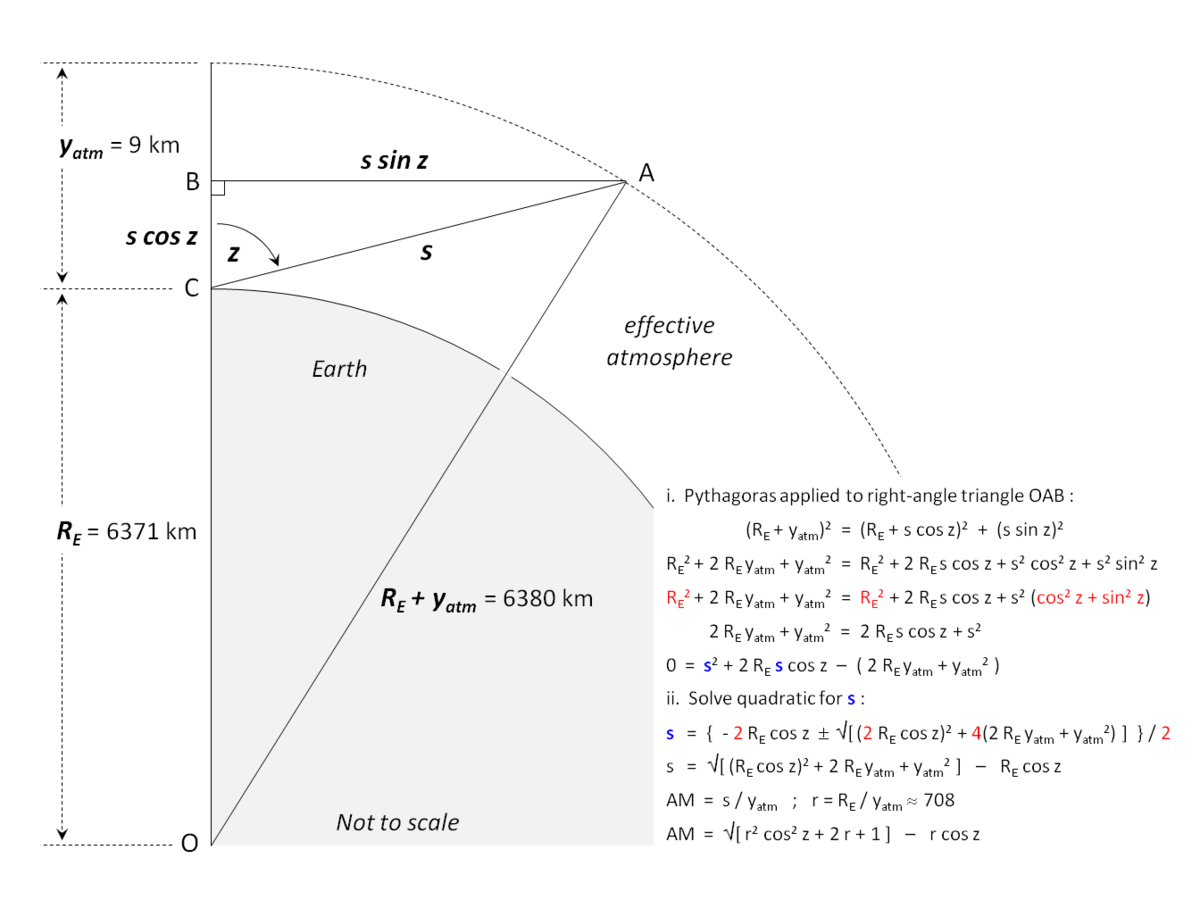
\includegraphics[width=0.6\linewidth]{../fig/Airmass_geometry.png}
		\caption{تغییر هندسی ستون جو با زاویه دید.}
	\end{figure}
	با توجه به قانون بیِر--لَمبِرت\footnote{\lr{Beer--Lambert}}، میزان نور عبوری از یک سیال با ضخامت آن به صورت
	نمایی افت می‌کند. بنابراین، قدر متناسب با ضخامت جو بین ناظر و ستاره افزایش می‌کند. اگر انحنای زمین را ناچیز
	فرض کنیم، ضخامت جو بین ستاره و ناظر، که آن را ستون جو می‌نامیم، متناسب است با $\sec z$ که $z$ زاویه ستاره
	با سرسو است. بنابراین
	\begin{equation}
		\text{قدر مشاهده‌شده} = ثابت + k\sec{z}
	\end{equation}
	که $k$ ضریب جذب جو است. با کم کردن $k\sec{z}$ از قدر ستاره، می‌توانیم آن‌ها را کالیبره کنیم، طوری که انگار
	همه ستاره‌ها را در سرسو مشاهده کرده‌ایم.
	\section{روش آزمایش}
	ابزار مورد استفاده ما در این آزمایش عبارت‌اند از:
	\begin{itemize}
		\item تلسکوپ نیوتنی هشت اینچی (بدون فیلتر)
		\item دوربین \lr{Canon EOS 1200D}
		\item مقر و موتور
	\end{itemize}
	محل رصد، روستای ازناوه واقع در نزدیکی شهر کاشان است. عکس‌ها با نوردهی $1.6$ ثانیه و \lr{ISO $1600$}
	در ساعت ۳۰:۱ تا ۲:۱۸ بامداد ۲۸ تیر ۱۴۰۲ گرفته شده‌اند. عکس‌هایی با نوردهی $1.6$ هم گرفته شده بود
	که به دلیل رَد داشتن قابل استفاده نیستند. پس از قطبی کردن و اطمینان از نوردهی، از خوشه دوتایی
	(خوشه‌های $\chi Persei$ و $h Persei$) با فاصله زمانی یک تا سه دقیقه عکس‌برداری کردیم. پس از رصد،
	در سپیده‌دم با عکس‌برداری بیرون از فکوس از آسمان، فریم‌های \lr{flat} را با نوردهی $2.5$ ثانیه و \lr{ISO $1600$}
	گرفتیم و در آخر با بستن دریچه دوربین و عکس‌برداری در نوردهی و \lr{ISO}های مربوطه، فریم تاریک و
	فریم تاریک \lr{flat} را گرفتیم. برای محاسبه ارتفاع ستاره‌ها در آسمان، از نرم افزار \lr{Starry Night} استفاده کردیم.
	\begin{figure}
		\centering
		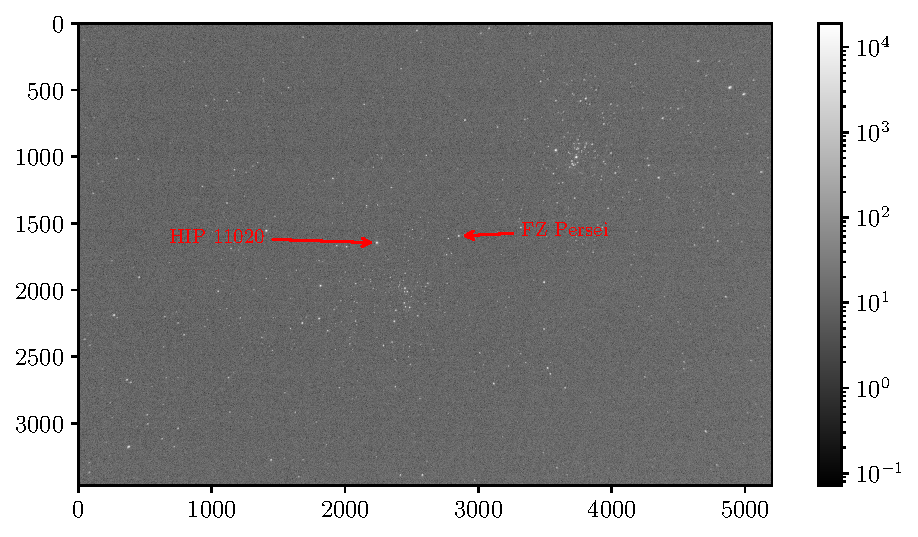
\includegraphics[width=\linewidth]{../fig/stars}
		\caption{یکی از عکس‌های گرفته شده بعد از انجام اصلاحات. مقادیر پیکسل‌ها به صورت لوگاریتمی بهنجار
			شده‌اند تا ستاره‌ها بهتر دیده شوند.}
	\end{figure}
	\section{اصلاح عکس‌ها}
	برای کم کردن جریان تاریک عکس، فریم تاریک با نوردهی مناسب (و میانه‌گرفته شده) را از عکس کم کردیم.
	سپس با تقسیم مقادیر پیکسل‌های عکس \lr{flat} بر میانه آن‌ها، \lr{gain table} را ساختیم و مقادیر پیکسل‌های
	عکس را بر مقادیر آن تقسیم کردیم تا عدم نوردهی یکنواخت پیکسل‌ها برطرف شود.
	
	سپس با مقایسه فریم تاریک با دو نوردهی متفاوت، پیکسل‌های مرده را پیدا کردیم که از تحلیل نهایی حذف شده‌اند.
	برای پیدا کردن پیکسل‌های مرده، ابتدا پیکسل‌های «داغ» را پیدا می‌کنیم (پیکسل‌هایی که مقدار بیش از حد بالایی دارند).
	سپس نمودار مقدار ای پیکسل‌ها در دو نوردهی برحسب هم را رسم می‌کنیم. اگر پیکسل‌ها مرده نباشند، باید روی یک خط
	گذرنده از مبدأ قرار بگیرند. این بدان معنی است که مقدار این پیکسل‌ها برحسب نوردهی قابل پیشبینی است که یعنی
	پاسخ نوری پیکسل‌ها سالم است. به دلیل وجود داده‌های پرت، نمی‌توانیم به پیکسل‌ها خط فیت کنیم، و از طرفی به دلیل
	وجود بایاس، شیب خط دقیقاً برابر با نسبت نوردهی‌ها نیست. بنابراین مجبوریم با سعی و خطا شیب خط را پیدا کنیم که
	زیاد سخت نیست. پس از رسم خط، پیکسل‌هایی که بیش از ۲۰ درصد با این خط فاصله دارند را به عنوان پیکسل مرده در نظر
	می‌گیریم. دقت کنید که پیکسل‌هایی که مقدار به نسبت کمتری دارند (از بقیه به وضوح جدا هستند) شامل این قاعده نمی‌شوند
	و آن‌ها را با یک مرز جدا می‌کنیم.
	
	در آخر، برای تحلیل داده ساده‌تر، با نسبت‌های مناسب سه کانال رنگی را ترکیب کردیم تا تصویر سیاه و سفید شود.
	با توجه به اینکه فضای رنگی عکس‌های استفاده شده، \lr{sRGB} است، روشنایی نسبی برحسب سه کانال رنگی برابر است با
	\begin{equation}
		\text{\lr{grayscale intensity}} = 0.2126r + 0.7152g + 0.0722b.
	\end{equation}
	این اعداد مربوط به حساسیت چشم انسان است (چشم به رنگ سبز حساس‌تر است).
	\begin{figure}
		\centering
		\begin{subfigure}{0.49\linewidth}
			\centering
			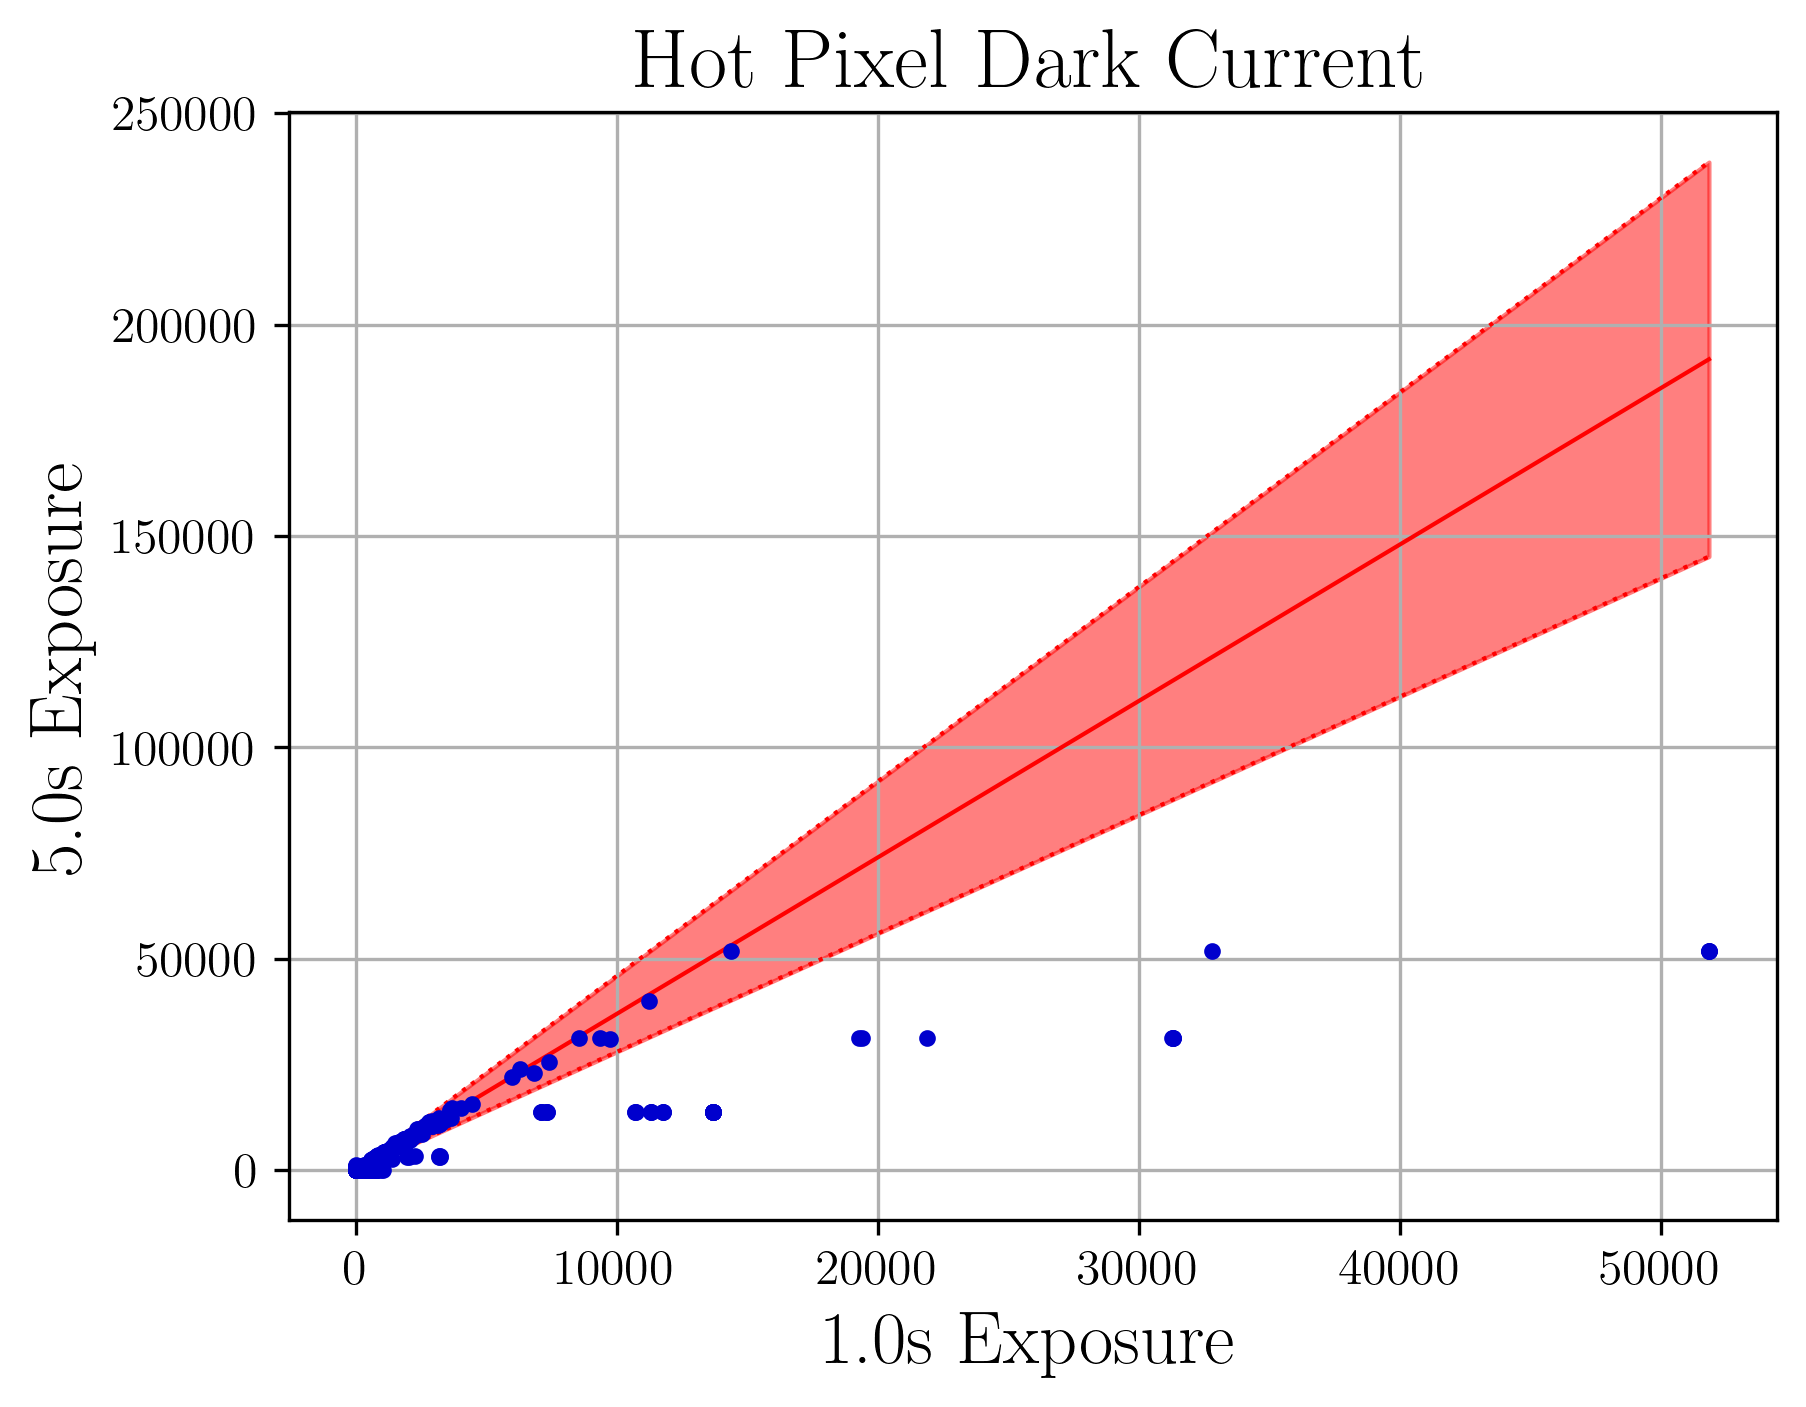
\includegraphics[width=\linewidth]{../fig/hotpix}
		\end{subfigure}
		\begin{subfigure}{0.49\linewidth}
			\centering
			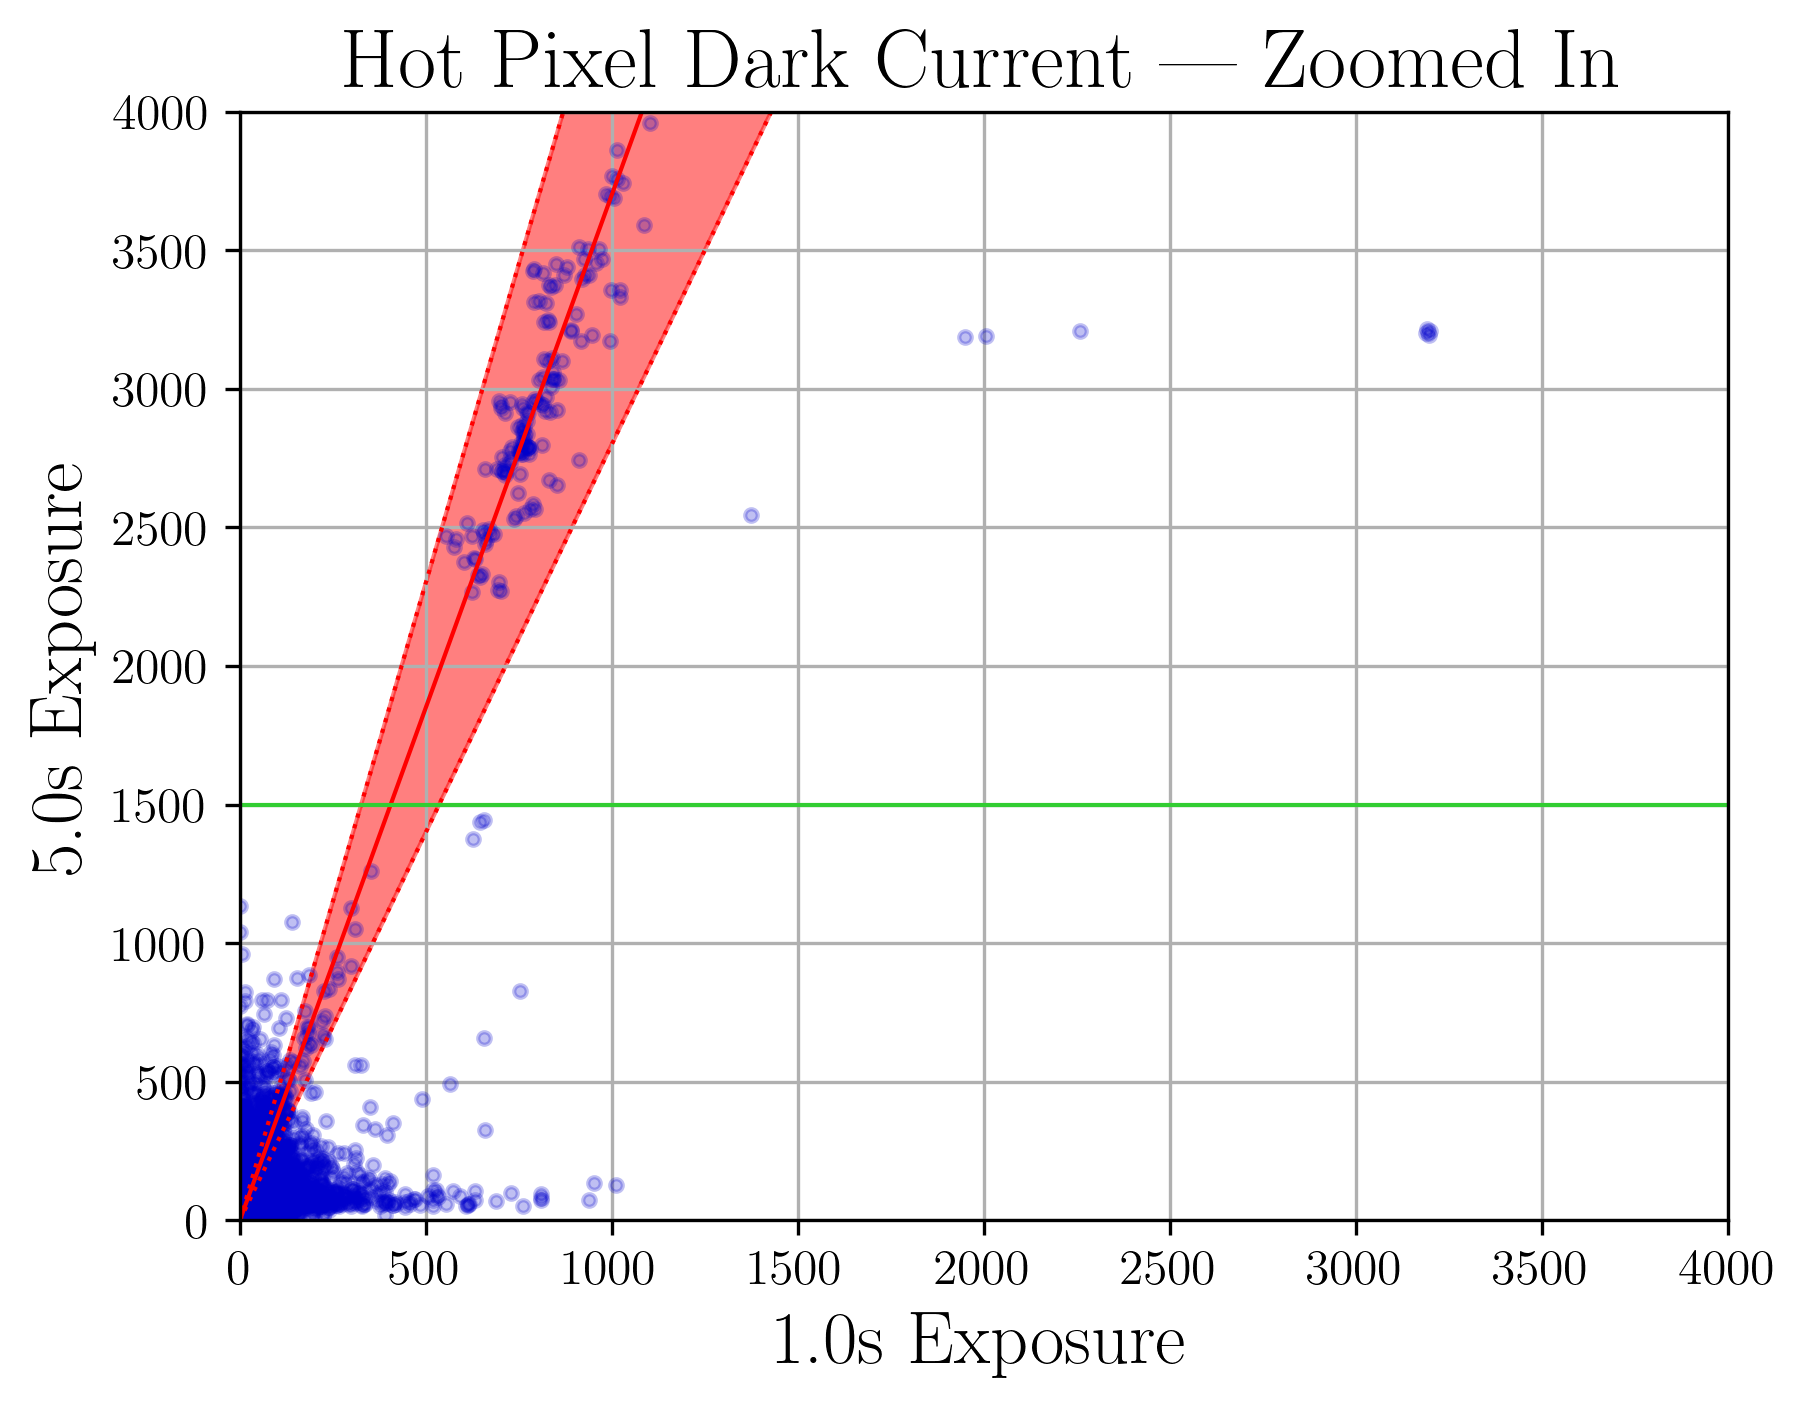
\includegraphics[width=\linewidth]{../fig/hotpix_zoom}
		\end{subfigure}
		\caption{نمودار پیکسل‌های داغ. پیکسل‌های خارج محدوده رنگی حذف می‌شوند.}
	\end{figure}
	\section{هم‌خط کردن عکس‌ها}
	برای اینکه بتوانیم یک ستاره خاص را دنبال کنیم، باید راهی پیدا کنیم که تصاویر را هم‌خط\footnote{\lr{align}} کنیم.
	برای این منظور، از پکیج \lr{\texttt{astroalign}} استفاده کردیم. این پکیج ابتدا ستاره‌ها را در دو تصویر پیدا می‌کند،
	سپس بین هر سه‌تا از آن‌ها مثلث می‌کشد و سعی می‌کند تبدیلی پیدا کند که یک تصویر را طوری به تصویر دیگر ببرد که این
	مثلث‌ها روی هم بیفتند. برای پیدا کردن مکان جدید ستاره، تبدیل عکس مرجع (یک عکس که در آن مکان ستاره را به‌طور دقیق
	پیدا کرده‌ایم) به هر عکس را پیدا می‌کنیم و مکان ستاره را تبدیل می‌کنیم.
	
	بعد از هم‌خط‌سازی اولیه، با الگوریتم \lr{DAOFIND} (نسخه پیاده‌سازی شده در پکیج \lr{\texttt{photutils}}) ستاره‌ها را
	پیدا می‌کنیم و نزدیک‌ترین ستاره در عکس به مکان تبدیل شده را پیدا می‌کنیم.
	
	روش‌های دیگری برای هم‌خط‌سازی براساس قدر ستاره‌ها وجود دارد، اما این روش‌ها دقت کمتری دارند. همچنین نرم‌افزار
	سیریل\footnote{\lr{Siril}} روش‌های متنوع‌تری دارد، اما ترجیح ما بر این بود که تمام مراحل داخل کُد پایتون انجام شود.
	\section{نورسنجی}
	برای نورسنجی از روش‌های متعددی استفاده کردیم که هیچکدام نتیجه مطلوبی ندادند.
	\begin{enumerate}
		\item نورسنجی دهانه. ستاره انتخاب‌شده منفرد است، پس می‌توان از این روش استفاده کرد
		\item نورسنجی \lr{psf} با استفاده از پکیج \lr{\texttt{photutils}}. در این روش یک تابع گوسی به هسته ستاره
		فیت می‌شود و شار آن برای محاسبه قدر، انتگرال این تابع است.
		\item شار کرنل گوسی تابع \lr{DAOFIND}. این روش دقت دو روش قبلی را ندارد و فقط برای تقریب اولیه استفاده می‌شود.
	\end{enumerate}

	\section{نتایج}
	\begin{figure}
		\centering
		\begin{subfigure}{0.49\linewidth}
			\centering
			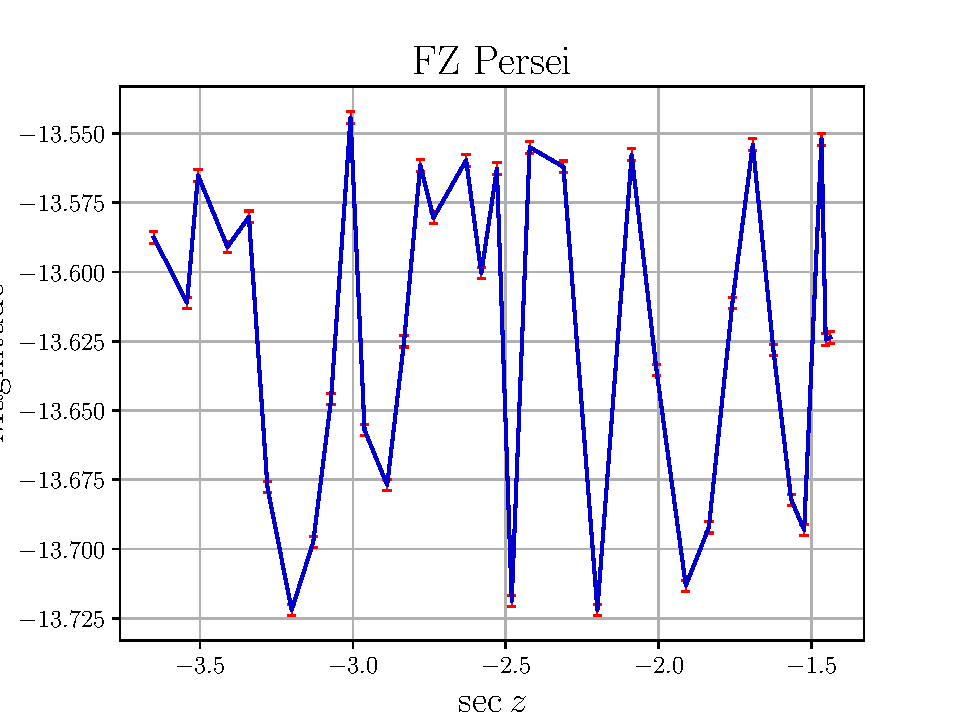
\includegraphics[width=\linewidth]{../fig/persei}
		\end{subfigure}
		\begin{subfigure}{0.49\linewidth}
			\centering
			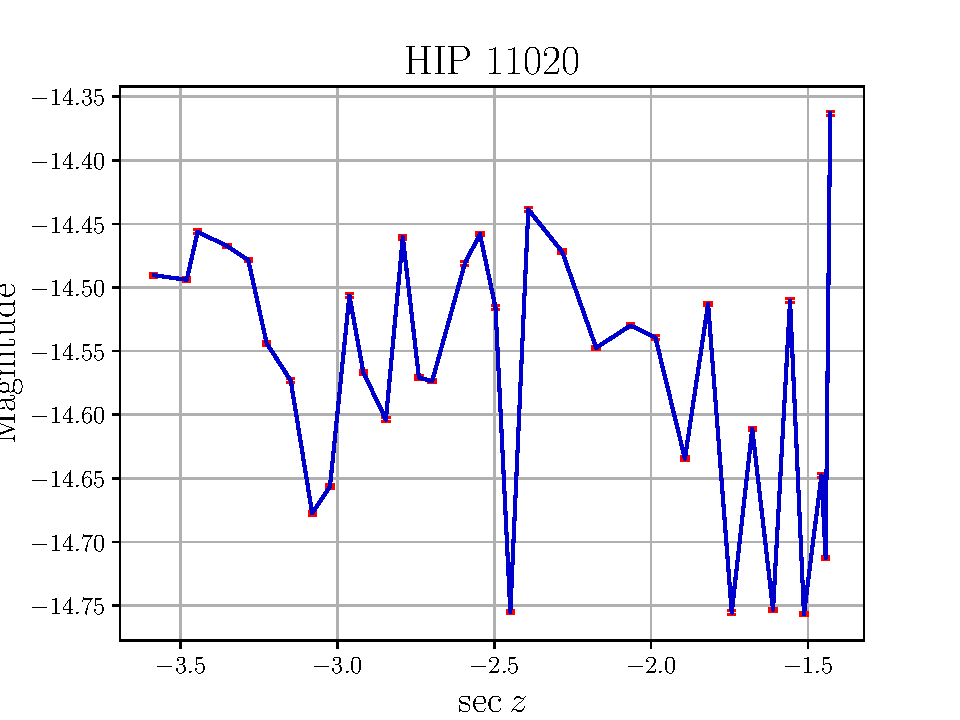
\includegraphics[width=\linewidth]{../fig/hip}
		\end{subfigure}
		\caption{قدر دو ستاره مختلف موجود در عکس. برای تحلیل نهایی از \lr{FZ Persei} استفاده کردیم.}
		\label{fig:raw}
	\end{figure}
	\begin{figure}
		\centering
		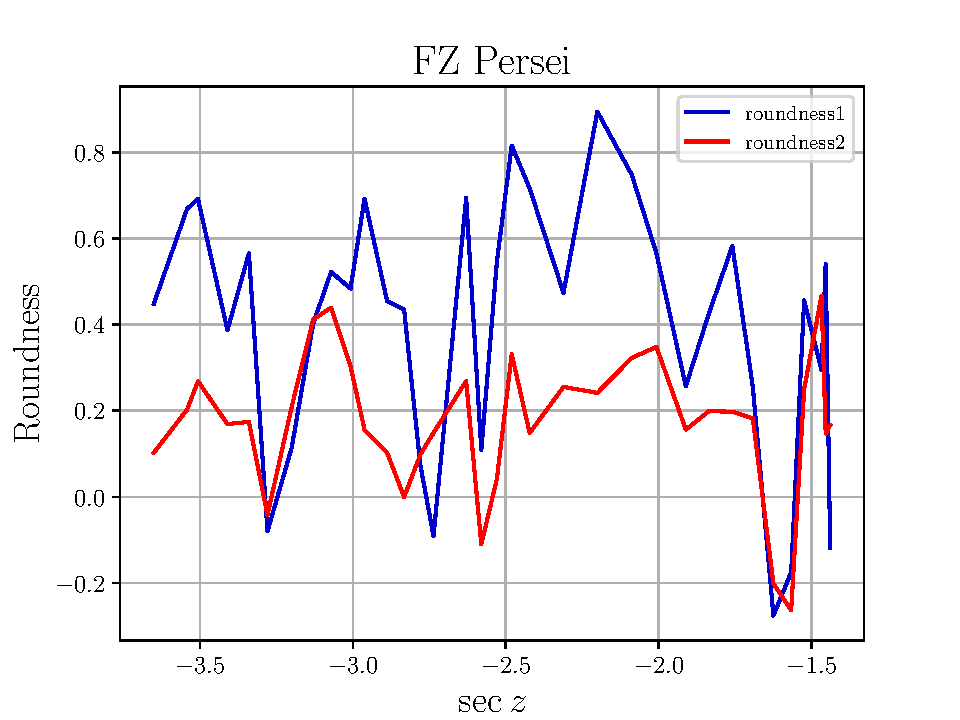
\includegraphics[width=\linewidth]{../fig/roundness}
		\caption{پارامترهای گِردی ستاره.}
		\label{fig:round}
	\end{figure}
	\begin{figure}
		\centering
		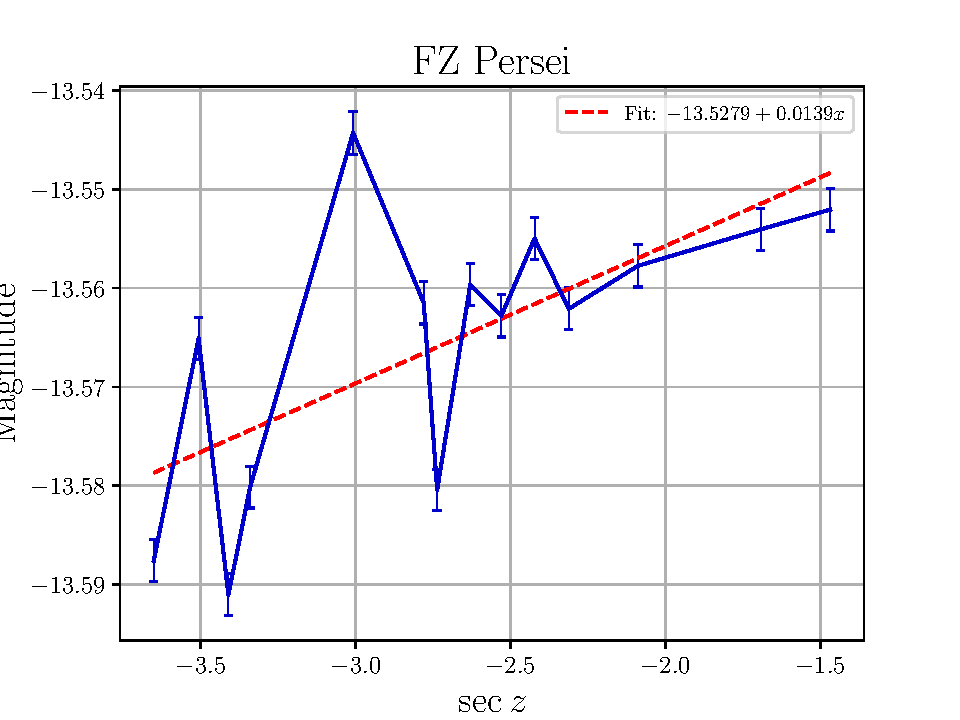
\includegraphics[width=\linewidth]{../fig/fit}
		\caption{خط فیت شده.}
	\end{figure}
	همان‌طور که در شکل \ref{fig:raw} مشاهده می‌کنید، همبستگی مناسبی بین زاویه $z$ و قدر ستاره وجود ندارد. این مشکل
	برای تمامی روش‌های نوردهی وجود داشت. با بررسی دقیق‌تر عکس‌ها، به نظر می‌رسد قدر‌های به نسبت کمتر مربوط به عکس‌هایی
	است که رَد دارند (هرچند بسیار کم). با توجه به شکل \ref{fig:round} این نقاط پارامترهای گِردی پایین‌تری نسبت به عکس‌های
	نزدیک به زمان خود دارند. در کل با حذف قدرهای از حدی کمتر (در اینجا برای \lr{FZ Persei} به اندازه $-13.6$) می‌توانیم
	این عکس‌ها را حذف کنیم.
	
	با وجود حذف داده‌های نامناسب، باز هم همبستگی بسیار کم است ($R^2 = 0.43 $) و عدد نهایی به سختی از نظر آماری معنادار
	است. ضریب جذب نهایی در بازه اطمینان ۹۵ درصد برابر
	\begin{equation}
		k = 0.014 \pm 0.01
	\end{equation}
	بدست آمده است.
\end{document}